% ============================================================
%  part5/ch26-coupled-functional.tex
%  Chapter 26: The Coupled RSVP Functional
% ============================================================

\chapter{The Coupled RSVP Functional}
\label{ch:coupled-functional}

\epigraph{%
  Dynamics follow from energy.\\
  Not vice versa.%
}{---}

\begin{WhyChapter}
  This is the mathematical heart of RSVP\@.
  Previous chapters introduced the individual fields and their
  roles.
  This chapter assembles the complete free-energy functional,
  derives all field equations, establishes boundedness below,
  and proves free-energy dissipation.
  Every subsequent cosmological prediction rests on the
  functional developed here.
\end{WhyChapter}


\begin{ChapterIntro}
Complex systems are often described by separate variables: density, flow, entropy, concentration, energy, order. In reality these quantities rarely evolve independently.

A change in one influences the others. Density alters transport. Transport alters entropy. Entropy alters stability. Stability alters subsequent transport.

The free-energy functional is an attempt to describe all of these influences within a single object. Rather than writing separate laws for separate quantities, the functional encodes the energetic cost of an entire configuration. Once such a functional exists, the equations of motion become consequences rather than assumptions. Dynamics emerge from the geometry of the energy landscape itself.
\end{ChapterIntro}

\section{The complete RSVP functional}

\begin{definition}[Complete RSVP free-energy functional]
  \label{def:complete-rsvp}
  \begin{align}
    \mathcal{F}[\Phi,\mathbf{v},S,\ell]
    &= \underbrace{\int_\Omega\frac{\alpha}{2}|\nabla\Phi|^2\,dx}_{\text{scalar gradient}}
    + \underbrace{\int_\Omega W(\Phi)\,dx}_{\text{scalar potential}}
    + \underbrace{\int_\Omega\frac{\beta}{2}|\nabla\ell|^2\,dx}_{\text{lamphron gradient}}
    \nonumber\\
    &\quad
    + \underbrace{\int_\Omega U(\ell)\,dx}_{\text{lamphron potential}}
    + \underbrace{\int_\Omega\lambda W(\Phi)\ell^2\,dx}_{\text{coupling}}
    + \underbrace{\int_\Omega\frac{\rho}{2}|\mathbf{v}|^2\,dx}_{\text{kinetic}}
    \nonumber\\
    &\quad
    + \underbrace{\int_\Omega\frac{\eta}{2}|\nabla\times\mathbf{v}|^2\,dx}_{\text{vorticity}}
    + \underbrace{\int_\Omega\frac{\chi}{2}|\nabla S|^2\,dx}_{\text{entropy gradient}}
    - \underbrace{\int_\Omega T S\,dx}_{\text{entropy source}}.
    \label{eq:full-rsvp-functional}
  \end{align}
\end{definition}

\subsection*{Term-by-term interpretation}

\begin{description}[leftmargin=3cm,style=nextline]
  \item[Scalar gradient $\frac{\alpha}{2}|\nabla\Phi|^2$]
    Penalises rapid spatial variation of $\Phi$.
    Creates interface energy between domains.
  \item[Scalar potential $W(\Phi)$]
    Double-well: $W(\Phi) = \frac{a}{2}\Phi^2 + \frac{b}{4}\Phi^4$
    with $a < 0 < b$ drives $\Phi$ toward $\pm\Phi_0$.
  \item[Lamphron gradient $\frac{\beta}{2}|\nabla\ell|^2$]
    Penalises sharp variation in lamphron amplitude.
    Stabilises coherent lamphron domains.
  \item[Lamphron potential $U(\ell)$]
    Constrains lamphron amplitude: e.g., $U(\ell) = \frac{c}{4}\ell^4$.
  \item[Coupling $\lambda W(\Phi)\ell^2$]
    Links scalar and lamphron fields.
    With $W \geq 0$ and $\lambda \geq 0$: bounded below.
    Physically: lamphron concentrates where $\Phi$ is structured.
  \item[Kinetic $\frac{\rho}{2}|\mathbf{v}|^2$]
    Kinetic energy of vector transport field.
  \item[Vorticity $\frac{\eta}{2}|\nabla\times\mathbf{v}|^2$]
    Penalises rotational flow; stabilises coherent transport.
  \item[Entropy gradient $\frac{\chi}{2}|\nabla S|^2$]
    Penalises sharp entropy gradients; drives entropy smoothing.
  \item[Entropy source $-TS$]
    Drives entropy toward higher values at rate $T$.
\end{description}

\section{Boundedness below}

\begin{theorem}[Functional boundedness]
  \label{thm:bounded-below}
  \statusproven{}
  Assume $W(\Phi) \geq 0$, $U(\ell) \geq 0$, $\lambda \geq 0$,
  and $T \leq 0$ (or $S$ bounded).
  Then $\mathcal{F} \geq 0$.
\end{theorem}

\begin{proof}
  Each of the first eight terms is nonnegative by assumption
  or by construction ($|\cdot|^2 \geq 0$, $\ell^2 \geq 0$,
  $W \geq 0$, $U \geq 0$, $\lambda \geq 0$).
  For the entropy source term: if $T \leq 0$ and $S \geq 0$,
  then $-TS \geq 0$.
  Alternatively if $S$ is bounded above by $S_{\max}$,
  one subtracts a constant.
  Therefore $\mathcal{F} \geq 0$ (or $\mathcal{F} \geq -TS_{\max}|\Omega|$).
\end{proof}

\begin{corollary}[Free-energy descent cannot diverge]
  Since $\mathcal{F}$ is bounded below, gradient flow solutions
  satisfy $\mathcal{F}(t) \geq \mathcal{F}(\infty) > -\infty$.
  The functional cannot descend to $-\infty$.
\end{corollary}

This corollary underlies all well-posedness arguments in
Part~IV and the cosmological stability claims in Part~VII.

\section{All variational derivatives}

\begin{theorem}[Complete variational derivatives]
  \label{thm:all-variations}
  \statusproven{}
  Under periodic or no-flux boundary conditions:
  \begin{align}
    \frac{\delta\mathcal{F}}{\delta\Phi}
    &= -\alpha\Delta\Phi + W'(\Phi) + \lambda W'(\Phi)\ell^2,
    \label{eq:var-Phi}\\
    \frac{\delta\mathcal{F}}{\delta\ell}
    &= -\beta\Delta\ell + U'(\ell) + 2\lambda W(\Phi)\ell,
    \label{eq:var-ell}\\
    \frac{\delta\mathcal{F}}{\delta S}
    &= -\chi\Delta S - T,
    \label{eq:var-S}\\
    \frac{\delta\mathcal{F}}{\delta\mathbf{v}}
    &= \rho\mathbf{v} + \eta\nabla\times(\nabla\times\mathbf{v}).
    \label{eq:var-v}
  \end{align}
\end{theorem}

\begin{proof}
  Each follows by the standard variational calculation:
  vary the respective field, integrate by parts, and collect
  the coefficient of the test function.
  Equation~\eqref{eq:var-Phi}: the $W(\Phi)\ell^2$ coupling
  contributes $\lambda W'(\Phi)\ell^2$ by the product rule.
  Equation~\eqref{eq:var-ell}: the coupling contributes
  $2\lambda W(\Phi)\ell$ by differentiating $\ell^2$.
  Equations~\eqref{eq:var-S} and~\eqref{eq:var-v} follow
  analogously.
\end{proof}

\section{The RSVP gradient-flow equations}

\begin{definition}[Full gradient-flow RSVP system]
  \label{def:rsvp-gf-full}
  \begin{align*}
    \partial_t\Phi + \mathbf{v}\cdot\nabla\Phi
    &= M_\Phi[\alpha\Delta\Phi - W'(\Phi) - \lambda W'(\Phi)\ell^2],\\
    \partial_t\ell + \mathbf{v}\cdot\nabla\ell
    &= M_\ell[\beta\Delta\ell - U'(\ell) - 2\lambda W(\Phi)\ell],\\
    \partial_t S + \mathbf{v}\cdot\nabla S
    &= M_S(\chi\Delta S + T) + \sigma,\\
    \rho(\partial_t\mathbf{v} + \mathbf{v}\cdot\nabla\mathbf{v})
    &= -M_v[\rho\mathbf{v} + \eta\nabla\times(\nabla\times\mathbf{v})]
      - \nabla p + \nu\Delta\mathbf{v}.
  \end{align*}
\end{definition}

\section{Second variation and stability}

\begin{theorem}[Stability via second variation]
  \label{thm:stability-2nd-var}
  \statusproven{}
  An equilibrium $(\Phi_0,\ell_0,S_0,\mathbf{v}_0)$ is
  linearly stable iff $\delta^2\mathcal{F} > 0$.
\end{theorem}

\begin{proof}
  Compute the Hessian matrix $H_f = (\partial^2 f/\partial u_i\partial u_j)$
  evaluated at equilibrium, where $u = (\Phi,\ell,S,\mathbf{v})$.
  Then $\delta^2\mathcal{F} = \int \delta U^T H_f\,\delta U\,dx$.
  By the spectral theorem, $\delta^2\mathcal{F} > 0$ for all
  $\delta U \neq 0$ iff $H_f$ is positive definite.
  By Sylvester's criterion: $H_f > 0$ iff all leading principal
  minors $\Delta_i > 0$.
\end{proof}

\begin{proposition}[Stability conditions on coupling]
  \label{prop:stability-coupling}
  For the coupling term $\lambda W(\Phi)\ell^2$,
  the Hessian contribution is
  $\begin{pmatrix}
    \lambda W''(\Phi_0)\ell_0^2 & 2\lambda W'(\Phi_0)\ell_0 \\
    2\lambda W'(\Phi_0)\ell_0 & 2\lambda W(\Phi_0)
  \end{pmatrix}$.
  Positive definiteness requires
  $\lambda W(\Phi_0) > 0$ and
  $2\lambda^2 W(\Phi_0)W''(\Phi_0)\ell_0^2 > 4\lambda^2 W'(\Phi_0)^2\ell_0^2$.
\end{proposition}

\section{Energy dissipation}

\begin{theorem}[RSVP energy dissipation]
  \label{thm:rsvp-dissipation-full}
  \statusproven{}
  For the gradient-flow RSVP system with incompressible
  transport and admissible entropy production,
  \[
    \frac{d\mathcal{F}}{dt}
    \leq -M_\Phi\!\int\!\Bigl|\frac{\delta\mathcal{F}}{\delta\Phi}\Bigr|^2 dx
    - M_\ell\!\int\!|\nabla\mu_L|^2 dx
    - \chi M_S\!\int\!(\Delta S)^2 dx \leq 0.
  \]
\end{theorem}

\begin{proof}
  Decompose $\frac{d\mathcal{F}}{dt}$ into advective and
  dissipative parts.
  For incompressible $\mathbf{v}$, the advective part vanishes.
  Each dissipative term has the form
  $-M_q\int|\delta\mathcal{F}/\delta q|^2\,dx \leq 0$.
  The entropy term contributes $-M_S\int(\Delta S)^2 dx$
  after integration by parts.
\end{proof}

\begin{StatusBox}{Proven Framework}
  Theorems~\ref{thm:bounded-below},~\ref{thm:all-variations},
  and~\ref{thm:rsvp-dissipation-full} together constitute the
  proven variational foundation of RSVP\@.
  Global existence of solutions (Conjecture~\ref{conj:rsvp-existence})
  remains open.
\end{StatusBox}

\begin{ProblemSet}
\problem{
  Show that $\mathcal{F}$ is bounded below by $-|T|S_{\max}|\Omega|$
  when $S \leq S_{\max}$.
  What does this bound imply for long-time behaviour?
}
\problem{
  For the coupling term $\lambda W(\Phi)\ell^2$ with
  $W(\Phi) = \Phi^2$:
  (a) Compute $\delta\mathcal{F}/\delta\Phi$ and $\delta\mathcal{F}/\delta\ell$.
  (b) Show that the coupling drives $\ell$ to grow where $\Phi^2$ is large.
  (c) Interpret physically: what does lamphron concentrate near?
}
\problem{
  Verify Proposition~\ref{prop:stability-coupling} for the
  specific case $W(\Phi) = \Phi^2$, $\Phi_0 = 1$, $\ell_0 = 1$.
  What constraint on $\lambda$ ensures positive definiteness?
}
\problem{
  \textbf{Open problem.}
  Prove or disprove: for any smooth initial data in $H^2(\Omega)$,
  the Allen--Cahn subsystem
  $\partial_t\Phi = M_\Phi[\alpha\Delta\Phi - W'(\Phi)]$
  admits a unique global smooth solution.
  State the precise functional-analytic conditions on $W$
  required for your argument.
}
\end{ProblemSet}

\section{Boundedness with coupling: explicit estimate}

\begin{theorem}[Lower bound with coupling]
  \label{thm:bounded-coupling}
  \statusproven{}
  Assume $\alpha,\beta,\chi,\lambda \geq 0$,
  $W(\Phi) \geq 0$, and potentials $V,U,Q \geq -C$ for some
  finite constant $C \geq 0$.
  Then
  \[
    \mathcal{F}[\Phi,\mathbf{v},S,\ell]
    \geq -3C|\Omega|.
  \]
\end{theorem}

\begin{proof}
  Since $\lambda \geq 0$ and $W(\Phi)\ell^2 \geq 0$:
  the coupling term is nonnegative.
  The gradient terms $|\nabla\Phi|^2$, $|\nabla\ell|^2$,
  $|\nabla S|^2$, $|\mathbf{v}|^2$, $|\nabla\times\mathbf{v}|^2$
  are all nonnegative.
  The three potential terms satisfy $V \geq -C$, $U \geq -C$,
  $Q \geq -C$.
  Therefore $\mathcal{F} \geq -3C|\Omega|$.
\end{proof}

\begin{corollary}[Dynamics cannot descend to $-\infty$]
  Since $\mathcal{F}$ is bounded below by $-3C|\Omega|$,
  gradient-flow solutions satisfy $\mathcal{F}(t) \geq -3C|\Omega|$
  for all $t \geq 0$.
  Free-energy descent has a floor.
\end{corollary}

This corollary is the analytic foundation for all stability
and long-time behaviour results in Parts~V and~VII\@.

% ---- Figures ------------------------------------------------

\begin{figure}[ht]
\centering
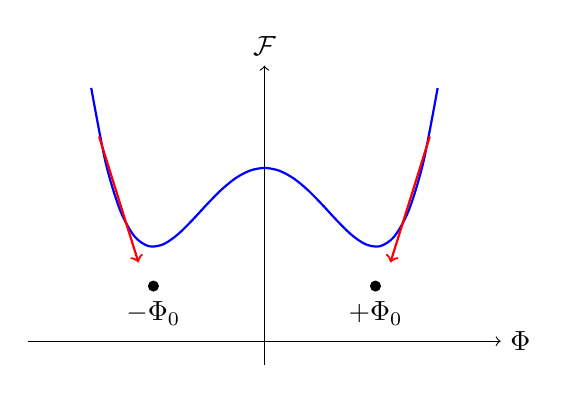
\begin{tikzpicture}
  \draw[->] (-3,0)--(3,0) node[right] {$\Phi$};
  \draw[->] (0,-0.3)--(0,3.5) node[above] {$\mathcal{F}$};
  \draw[domain=-2.2:2.2,smooth,thick,blue]
    plot(\x,{0.25*(\x)^4 - (\x)^2 + 2.2})
    node[above right,blue] {};
  % Minima markers
  \fill (-1.41,0.7) circle (2pt);
  \fill ( 1.41,0.7) circle (2pt);
  \node at (-1.41,0.35) {$-\Phi_0$};
  \node at ( 1.41,0.35) {$+\Phi_0$};
  % Gradient flow arrows
  \draw[->,thick,red] (-2.1,2.6) -- (-1.6,1.0);
  \draw[->,thick,red] ( 2.1,2.6) -- ( 1.6,1.0);
\end{tikzpicture}
\caption{Typical RSVP free-energy landscape for the $\Phi$ sector.
         The double-well potential $W(\Phi)$ creates two stable
         phases $\Phi = \pm\Phi_0$.
         Gradient-flow trajectories (red arrows) descend toward
         the minima.}
\label{fig:rsvp-energy-landscape}
\end{figure}

\begin{CitationAnchor}
  The variational-derivative calculation
  (Theorem~\ref{thm:all-variations}) follows standard
  functional analysis; see Evans~\cite{evans2010} and
  Jost (2013) for the PDE theory.
  The Lyapunov-function methodology (Theorem~\ref{thm:rsvp-dissipation-full})
  is a standard tool in gradient-flow theory; see
  Temam~\cite{temam2001} for applications to
  Navier--Stokes type systems, and Jordan, Kinderlehrer \& Otto
  (1998) for the Wasserstein gradient-flow interpretation.
  The Hessian stability criterion follows the calculus of
  variations as in Zeidler (1985).
\end{CitationAnchor}

\begin{FurtherReading}
  The mathematical theory of gradient flows, including
  well-posedness and long-time behaviour, is treated in
  Evans~\cite{evans2010} (Chapter~8) and Temam~\cite{temam2001}.
  For the specific analysis of Allen--Cahn and Cahn--Hilliard
  as gradient flows, see the review by Fife (2000).
  The abstract gradient-flow framework in metric spaces
  is developed in Ambrosio, Gigli \& Savaré (2005).
\end{FurtherReading}
